\chapter{System operacyjny FreeRTOS}
\label{cha:freertos}

Podstawową częścią każdego systemu operacyjnego jest jego jądro, które odpowiedzialne jest za udostępnianie zasobów sprzętowych, takich jak procesor, pamięć  czy urządzenia wejścia/wyjścia programom wykonywanym na tym systemie.

System FreeRTOS jest mikrojądrem (por. architektury oprogramowania na str. \pageref{ref:architektury}), przy użyciu którego możliwa jest implementacja aplikacji czasu rzeczywistego (zarówno o miękkich jak i twardych wymaganiach) na urządzeniach wbudowanych.

W niniejszym rozdziale opisano architekturę systemu (mikrojądra) FreeRTOS wraz ze sposobem, w jaki
poszczególne funkcjonalności mogą być przydatne w implementacji maszyny wirtualnej Erlanga dedykowanej dla tego systemu.

%---------------------------------------------------------------------------
\section{Zadania i planista (\emph{scheduler})}
\label{sec:rtosScheduler}

Podstawową wykonywalną jednostką w systemie FreeRTOS jest zadanie, zarządzane przez wbudowanego w system planistę (\emph{scheduler}).
Zadanie uruchomione pod nadzorem planisty można porównać do wątku w systemie Linux, z tą różnicą, że kod zadania musi zostać zaimplementowany w języku C~i~przed rozpoczęciem jego wykonywania należy zadeklarować rozmiar stosu danego zadania.

Zadaniom można również nadawać priorytety. Jeżeli do wykonania przeznaczone są zadania o różnych priorytetach, to w pierwszej kolejności wykonane zostanie to o wyższym priorytecie. W bardzo podobny sposób działa algorytm kolejkowania procesów w maszynie wirtualnej BEAM.

Samo zadanie można znajdować się w kilku stanach w zależności m.in. od tego, czy planista wybrał je do wykonania, czy dopiero oczekuje ono na swoją kolej. Pełny diagram stanów, w jakich może znajdować się zadanie w systemie FreeRTOS zaprezentowany został na rysunku \ref{fig:taskstate}.

\begin{figure}[h]
\centerline{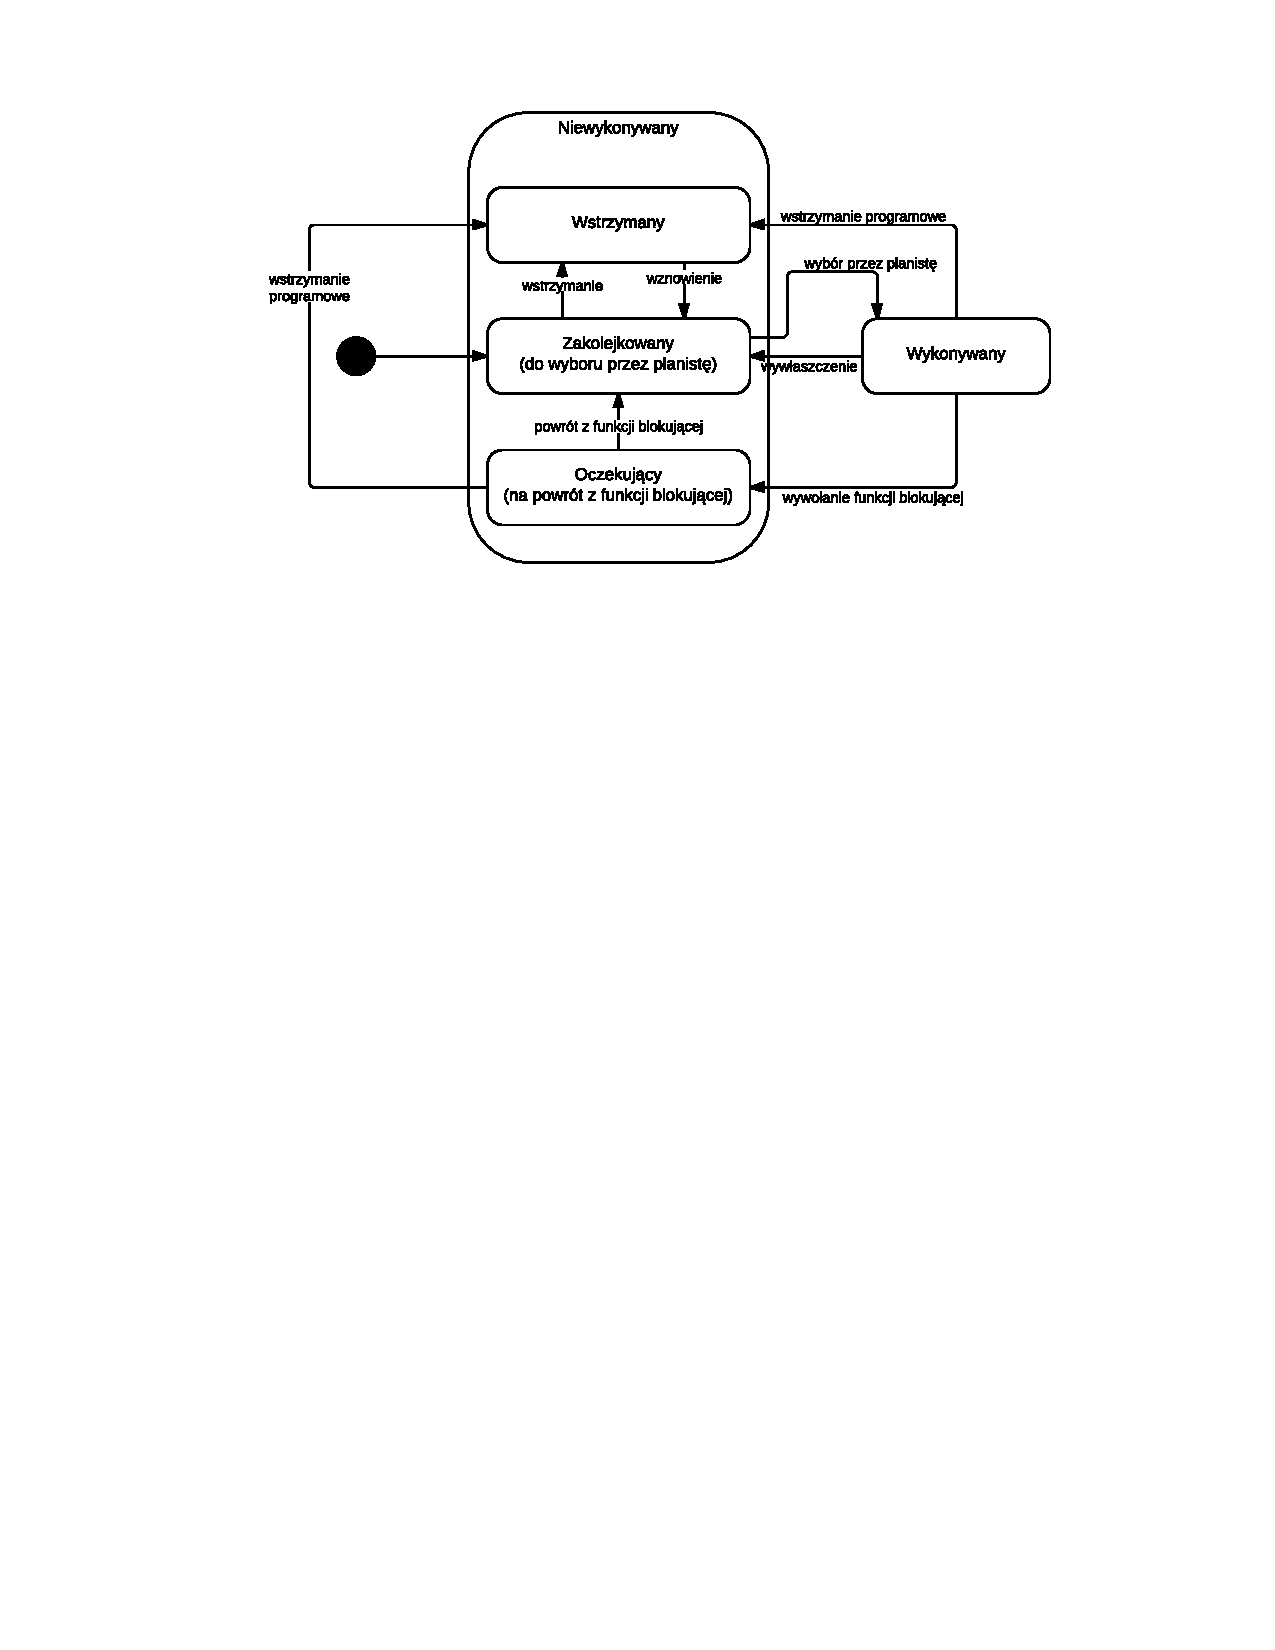
\includegraphics[scale=1, clip, trim=0 180mm 0 15mm]{freertos_task_state}}
\caption{Diagram stanów zadania w systemie FreeRTOS}
\label{fig:taskstate}
\end{figure}


\emph{Scheduler} może pracować w dwóch trybach: wywłaszczeniowym, w którym sam algorytm planisty decyduje o kolejności wykonywania zadań, oraz w trybie opartym na współpracy, w którym zadania ,,dobrowolnie'' rezygnują z czasu procesora, który został im przydzielony. W tym drugim przypadku priorytety zadań są nadal brane pod uwagę podczas wyboru kolejnego zadania do wykonania.

Wielozadaniowość oparta na współpracy to model, jaki został zaimplementowany w oryginalnej maszynie wirtualnej Erlanga, po wprowadzeniu pojęcia redukcji jako miary czasu, przez jaki danemu procesowi udostępniona jest moc obliczeniowa (por. podrozdział \ref{sec:maszynaScheduler}).

Wymienione cechy charakterystyczne zadań i planisty stanowiły bardzo dobry punkt wyjścia do oparcia implementacji \emph{schedulera} maszyny wirtualnej Erlanga na planiście systemu FreeRTOS oraz enkapsulację logiki procesów w zadaniach.

%---------------------------------------------------------------------------
\section{Kolejki}
\label{sec:rtosKolejki}

System FreeRTOS zapewnia mechanizm kolejki wiadomości między procesami, na wzór kolejki wiadomości POSIX. Kolejki nie należą do żadnego z zadań, dlatego też każde z zadań może zarówno odczytywać jak i zapisywać dane do każdej z nich. Proces przesłania i odebrania wiadomości polega na skopiowaniu danych z przestrzeni adresowej zadania-nadawcy do przestrzeni adresowej kolejki a~następnie z przestrzeni adresowej kolejki do przestrzeni adresowej zadania-adresata.

Kolejki w systemie FreeRTOS bardzo dobrze oddają semantykę kolejki wiadomości (\emph{mailbox}) w~procesie erlangowym. Jednakże, aby oprzeć na nich implementację tej funkcjonalności, istniałaby konieczność utworzenia osobnej kolejki dla każdego z uruchomionych w systemie procesów, do czego konieczne jest z góry zaalokowanie pamięci dla kolejki wiadomości o maksymalnej długości.

W związku z tym, w maszynie wirtualnej opisanej w niniejszej pracy kolejki wiadomości zostały zaimplementowane wewnątrz zadań implementujących logikę procesów. Pozwoliło to na uproszczenie procedury wysłania wiadomości do procedury przez umieszczenie wiadomości na stercie procesu będącego jej adresatem, z której proces będzie mógł korzystać aż do momentu odśmiecenia pamięci procesu. 

%---------------------------------------------------------------------------
\section{Przerwania}
\label{sec:rtosPrzerwania}

FreeRTOS zapewnia obsługę zarówno programowych jak i sprzętowych przerwań. Podejściem do implementacji obsługi przerwań, który zalecany jest przez autorów systemu jest ich odroczenie i delegacja obsługi do innego zadania, niż to obsługujące przerwanie (\emph{Interrupt Service Routine} - ISR) \cite{Barry2011}. Motywacją do tego, aby kod ISR był możliwie jak najkrótszy jest fakt, że w momencie jego wykonywania nowe przerwania nie są wykrywane.

W implementacji maszyny wirtualnej Erlanga dla FreeRTOS podążono za tą koncepcją i informacja o przerwaniu jest przesyłana jako wiadomość do procesów, które wywołały wcześniej odpowiednią wbudowaną funkcję subskrybującą. Efektem takiego wywołania jest zgłoszenie maszynie wirtualnej, że dany proces jest ,,zainteresowany'' otrzymywaniem wiadomości dotyczących przerwań danego rodzaju. 

%---------------------------------------------------------------------------
\section{Zarządzanie zasobami}
\label{sec:rtosZasoby}

W systemach, które pozwalają na działanie wielu zadań współbieżnie niezbędna jest obecność mechanizmów pozwalających na 
zarządzanie dostępem do pewnych obszarów pamięci. W sytuacji, gdy dwa współbieżne zadania (np. zadanie obsługujące przerwanie i 
zadanie implementujące logikę procesu) będą modyfikować pewien obszar pamięci w sposób nieatomiczny i jedno z zadań zostanie wywłaszczone w momencie, gdy cała operacja nie zostanie zakończona, obszar pamięci pozostanie w stanie niespójnym.

FreeRTOS zapewnia następujące mechanizmy do synchronizacji zadań:
\begin{itemize}
\item \textbf{sekcja krytyczna} - powoduje zablokowanie dostępu do czasu procesora dla wszystkich pozostałych zadań, możliwe jest także zablokowanie obsługi pewnego rodzaju przerwań;
\item \textbf{mutex} - pozwalający na synchronizację dostępu do dzielonego zasobu przez ,,zainteresowane'' zadania, które muszą uzyskać dostęp do mutexu. Ma do tego prawo tylko jedno zadanie w jednym czasie, przed wykonaniem operacji na dzielonym zasobie;
\item \textbf{semafor} - działający jak mutex, pozwalający na dostęp większej liczby zadań do zasobu, jest zablokowany gdy jego wartość jest równa 0. Mutex jest szczególnym przypadkiem semafora, mogącym przyjąć tylko wartość 0 lub 1. W systemie FreeRTOS zarówno mutex jak i semafor zaimplementowane są przy użyciu tych samych struktur danych.
\end{itemize}

Wymienione mechanizmy synchronizacji zostały wykorzystane w elementach maszyny wirtualnej, w których było to konieczne, głównie w przypadku operacji wejścia-wyjścia.
Należy wspomnieć, że ze względu na rozważany typ maszyny (uruchamianej na procesorze o jednym rdzeniu) jak i również ze względu na model wielozadaniowości oparty na współpracy, udało się uniknąć użycia mechanizmów synchronizacji w wielu miejscach, w których intuicja podpowiadałby ich użycie.

%---------------------------------------------------------------------------
\section{Zarządzanie pamięcią}
\label{sec:rtosPamiec}

FreeRTOS udostępnia, spójny dla wszystkich swoich portów, interfejs do zarządzania pamięcią, składający się z dwóch funkcji: \texttt{pvPortMalloc()} oraz \texttt{vPortFree()} będące odpowiednikami funkcji systemowych \texttt{malloc()} i \texttt{free()}. 

Programista implementujący aplikację z użyciem mikrojądra FreeRTOS może wybrać jedną z czterech implementacji powyższych funkcji:
\begin{itemize}
\item \textbf{heap\_1} - która nie pozwala na zwolnienie raz zaalakowanej pamięci, przeznaczona do bardzo prostych aplikacji wbudowanych, w których liczba i rozmiar struktura jest z góry znana;
\item \textbf{heap\_2} - używająca algorytmu najlepszego dopasowania (\emph{best-fit}) do alokacji bloku pamięci, nie pozwala jednak na ponowne użycie dwóch sąsiednich, zwolnionych wcześniej bloków do zaalokowania nowego, większego bloku;
\item \textbf{heap\_3} - opakowująca wewnątrz sekcji krytycznej funkcje \texttt{malloc} i \texttt{free} udostępnianie przez kompilator, wadą tego rozwiązania jest duży rozmiar pliku wynikowego;
\item \textbf{heap\_4} - działająca jak \textbf{heap\_2}, rozwiązująca jednak problem alokacji pamięci w sąsiednich blokach.
\end{itemize}

Mając na uwadze fakt, że implementowane środowisko uruchomieniowe przeznaczone będzie dla języka z automatycznym zarządzaniem pamięcią, wraz ze wzrostem rozmiaru pamięci procesu algorytm \emph{garbage collectora} będzie potrzebował alokować coraz to większe bloki pamięci. Z tego powodu należało zwrócić szczególną uwagę na wybór strategii zapewniającą dobrą fragmentację dostępnej pamięci RAM, wybraną strategią zarządzania pamięcią do użycia w implementowanej maszynie wirtualnej została zatem implementacja \textbf{heap\_4}.

Oryginalna maszyna wirtualna Erlanga używa wielu różnych strategii alokowania pamięci, minimalizujących jej fragmentację, w zależności od przeznaczenia danego segmentu pamięci i jego rozmiaru. Maszyna rozważana w niniejszej pracy używa tylko ww. interfejsu udostępnionego przez FreeRTOS i~jemu powierza zadanie dobrego dopasowania alokowanych obszarów pamięci.

%---------------------------------------------------------------------------
\section{FreeRTOS i LPC176x}
\label{sec:rtosLPC}

Mikrojądro FreeRTOS zostało przeniesione na ponad 20 rodzin mikrokontrolerów, w tym na LPC1769, który zawiera procesor ARM Cortex-M3.

Mikrokontroler ten ma następujące parametry:
\begin{itemize}
\item 64 kB pamięci SRAM;
\item 512 kB pamięci flash;
\item posiada 4 interfejsy UART (\emph{Universal Asynchronous Receiver-Transmitter});
\item posiada 3 interfejsy I\textsuperscript{2}C / TWI (\emph{Two-Wire Interface});
\item posiada 1 interfejs SPI (\emph{Serial Peripherial Interface});
\item posiada 2 interfejsy SSP (\emph{Synchronous Serial Port});
\item posiada 2 interfejsy CAN (\emph{Controller Area Network});
\item posiada interfejs modulacji sygnału cyfrowego PWM (\emph{Pulse-Width Modulation});
\item posiada 1 interfejs USB 2.0 (\emph{Universal Serial Bus});
\item posiada 70 pinów ogólnego przeznaczenia GPIO (\emph{General Purpose Input-Output});
\item posiada 12-bitowy przetwornik analogowo-cyfrowy (ADC);
\item posiada 10-bitowy przetwornik cyfrowo-analogowy (DAC);
\item posiada cztery liczniki ogólnego przeznaczenia;
\item posiada zegar czasu rzeczywistego (RTC) z dedykowanym dla niego źródłem sygnału zegarowego.
\end{itemize}

Dokładne właściwości wymienionych wyżej elementów mikrokontrolera zawarte są w jego nocie katalogowej \cite{NXP2014}.

W sprzedaży dostępna jest tania płytka rozwojowa ze wspomnianym mikrokontrolerem, produkowana przez firmę NXP, posiadająca zintegrowany interfejs JTAG, służący do debugowania aplikacji. Wygląd takiego układu uruchomieniowego został zaprezentowany na rysunku \ref{fig:lpc1769}. Przez tę samą firmę udostępnianie jest również środowisko deweloperskie pozwalające na łatwą kompilację i debugowanie rozwijanego oprogramowania - LPCXpresso.

\begin{figure}[h]
\centerline{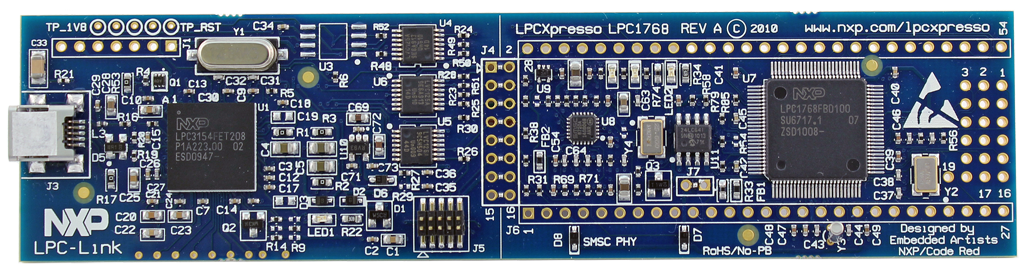
\includegraphics[scale=0.4]{lpc176x}}
\caption{Płytka rozwojowa z mikrokontrolerem LPC176x. Źródło: \url{http://www.embeddedartists.com/}}
\label{fig:lpc1769}
\end{figure}

Maszyna wirtualna opisywana w niniejszej pracy została rozwijana na ww. mikrokontrolerze, z~użyciem ww. narzędzi deweloperskich. Można założyć, że maszyna wirtualna Erlanga prezentowana w niniejszej pracy, po dopasowaniu działania niektórych funkcji wbudowanych do architektury odpowiedniego mikrokontrolera, będzie działać z portami systemu FreeRTOS również na inne platformach sprzętowych. Część z opisanych w pracy funkcjonalności, w szczególności dotyczących operacji wejścia-wyjścia, jest specyficzna dla wersji systemu dla mikrokontrolera LPC1769.

%---------------------------------------------------------------------------
\section{Podsumowanie}
\label{sec:rtosPodsumowanie}

Mikrojądro FreeRTOS udostępnia podstawowe mechanizmy do obsługi wielozadaniowości, komunikacji międzyprocesowej, zarządzania dostępem do zasobów współdzielonych oraz do zarządzania pamięcią. Są one jednak wystarczające do wykorzystania w implementacji maszyny wirtualnej Erlanga przeznaczonej dla systemu FreeRTOS.

Część z wymienionych wyżej funkcjonalności FreeRTOS jest na tyle zgodna z oryginalną maszyną wirtualną, że może zostać wykorzystana wprost do implementacji pewnych elementów maszyny. Część z nich musiała jednak ulec częściowej modyfikacji lub zostać całkowicie zaimplementowana, jak np. kolejki wiadomości procesów. 